\documentclass[letterpaper,12pt]{article}

\usepackage{geometry, pslatex, fancyhdr, graphicx}
\usepackage{amsmath,amsthm,amssymb,scrextend}
\usepackage{multicol}
\usepackage{tabularx}
\usepackage[makeroom]{cancel}
\usepackage{color}
\geometry{ margin = 1.0in }

%%% TODO modify these variables as per your homework %%%
\def\homeworknum{2}
\def\myname{Harshit Jain}
\def\myuserid{hmj5262}
%%%%

\pagestyle{fancy}
\lhead{{\bf CMPSC 464 Spring 2024}}
\chead{{\bf Assignment~\homeworknum}}
\rhead{{\bf \today}}
\let\newproof\proof
\renewenvironment{proof}{\begin{addmargin}[1em]{0em}\begin{newproof}}{\end{newproof}\end{addmargin}\qed}

\newcounter{problemid}
\stepcounter{problemid}
\def\newproblem{\clearpage\newpage{\bf Problem~\arabic{problemid}\stepcounter{problemid}}\hfill\par}

\setlength\parindent{0em} 
\setlength\parskip{8pt}
\setlength{\fboxsep}{6pt}


\begin{document}

\framebox[\textwidth]{
	\parbox{0.96\textwidth}{
		\parbox{0.12\textwidth}{\bf Name:}\parbox{0.6\textwidth}{\myname}\\
		\parbox{0.12\textwidth}{\bf User ID:}\parbox{0.6\textwidth}{\myuserid}
	}
}

%% your solutions %%%


% PROBLEM 1
\newproblem 

Proof by contradiction: assume that $L = \{w : w$ has balanced parentheses $\}$ is regular.

Then by the Pumping Lemma, there is some pumping length $n$, such that any word $w$ in $L$ of length at least $n$ can be split into $w = xyz$ satisfying the following conditions:
\begin{itemize}
    \item $|xy| \leq n$,
    \item $|y| > 0$,
    \item $xy^i z \in L$ for all $i > 0$.
\end{itemize}

We let $w$ be the word with $n$ left parentheses, followed by $n$ right parentheses. So, $w = (^n )^n$. Clearly, $w$ has balanced parentheses, so $w \in L$. 

Thus, since $|w| \geq n$, by the pumping lemma we must be able to write $w = xyyz$ with $|xy| \leq n$, $|y| \geq 1$, and such that $xy^i z \in L$ for all $i \geq 0$. However, since $w$ starts with $n$ $($'s, $y$ must consist entirely of one or more $($'s. Then by the first condition, we know that $y$ consists only of left parentheses. By the second condition, we know that $y$ is nonempty. So the string $xyyz$ must have more left parentheses than right parentheses.

Therefore, for any $i > 1$, $xy^i z \notin L$ since it has more $($'s than $)$'s. This is a contradiction, so $L$ is not regular.    

% PROBLEM 2
\newproblem
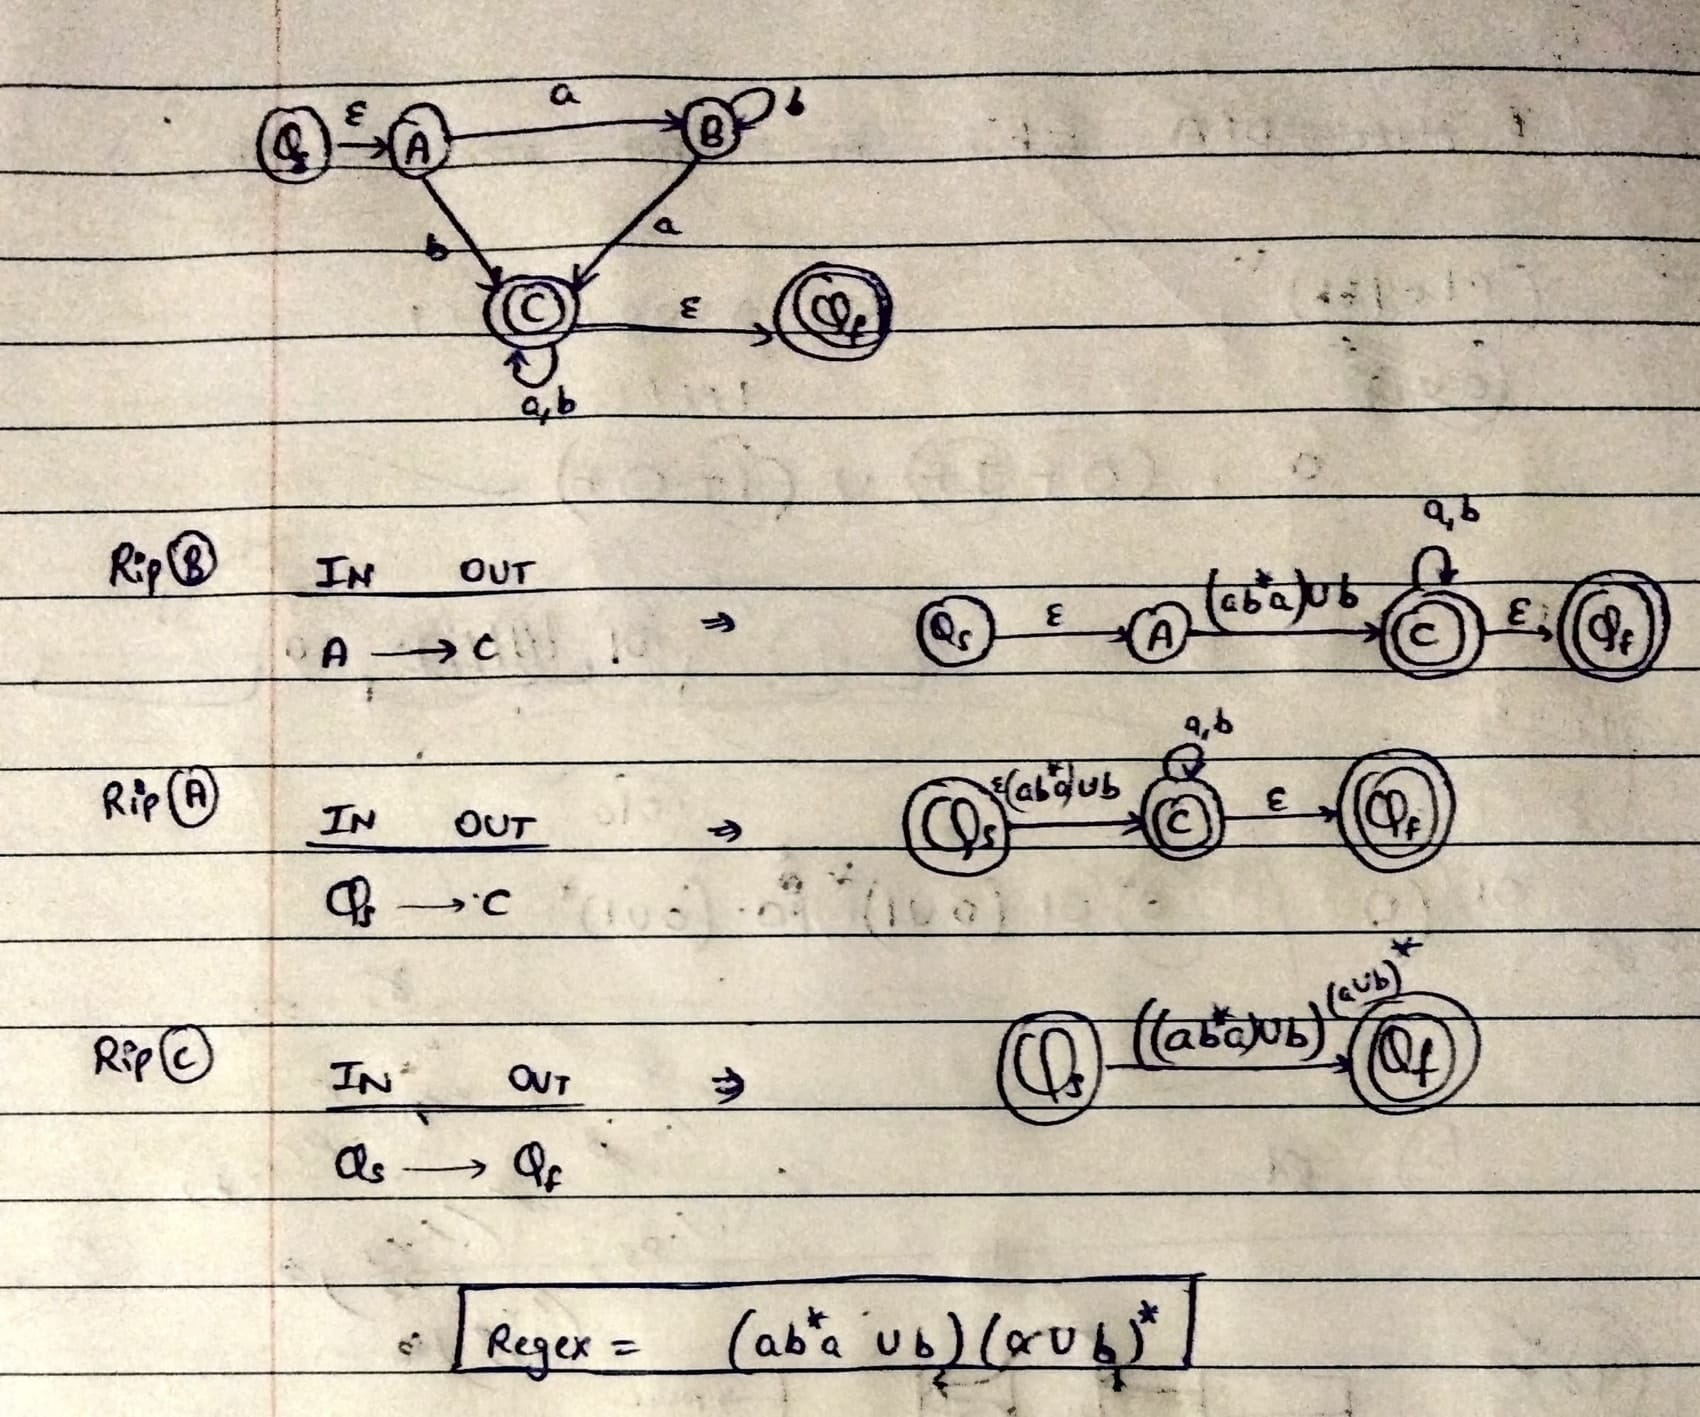
\includegraphics[scale = 0.20]{2}

% PROBLEM 3
\newproblem

\textbf{Proof:} We will use the Pumping Lemma for regular languages to prove that $L$ is not regular. The Pumping Lemma states that for any regular language $L$, there exists a constant $p$ (the pumping length) such that any string $s$ in $L$ with length at least $p$ can be split into three parts, $xyz$, satisfying the following conditions:

\begin{enumerate}
    \item For each $i \geq 0$, $xy^iz \in L$.
    \item $|y| > 0$ ($y$ is non-empty).
    \item $|xy| \leq p$.
\end{enumerate}

Now, assume for contradiction that the language $L$ is regular. Consider the string $s = {0}^p + {1}^p = {2}^p$ in $L$. According to the Pumping Lemma, we can write $s$ as $xyz$ such that the conditions are satisfied. Let $s = xyz$ where $|xy| \leq p$ and $|y| > 0$.

Since $|xy| \leq p$, the string $y$ can only consist of $0$s or $1$s (because the other characters in $\Sigma$ are '+', '=', and digits $2$ to $9$).

Now, consider the pumped string $s' = xy^2z$. Since $y$ is non-empty, the pumped string will have more $0$s or $1$s than the original string. Now, let's analyze $s'$ in terms of the given language $L$. The equation "$a+b=c$" implies that the number of occurrences of the digit '0' should be equal to the number of occurrences of the digit '1'. However, pumping $y$ will disturb this balance, leading to a string that does not satisfy the equation in $L$.

Therefore, $s' = xy^2z$ is not in $L$, which contradicts the Pumping Lemma. As a result, our initial assumption that $L$ is regular is false.

Hence, we can conclude that the language $L$ is not regular.

% PROBLEM 4
\newproblem
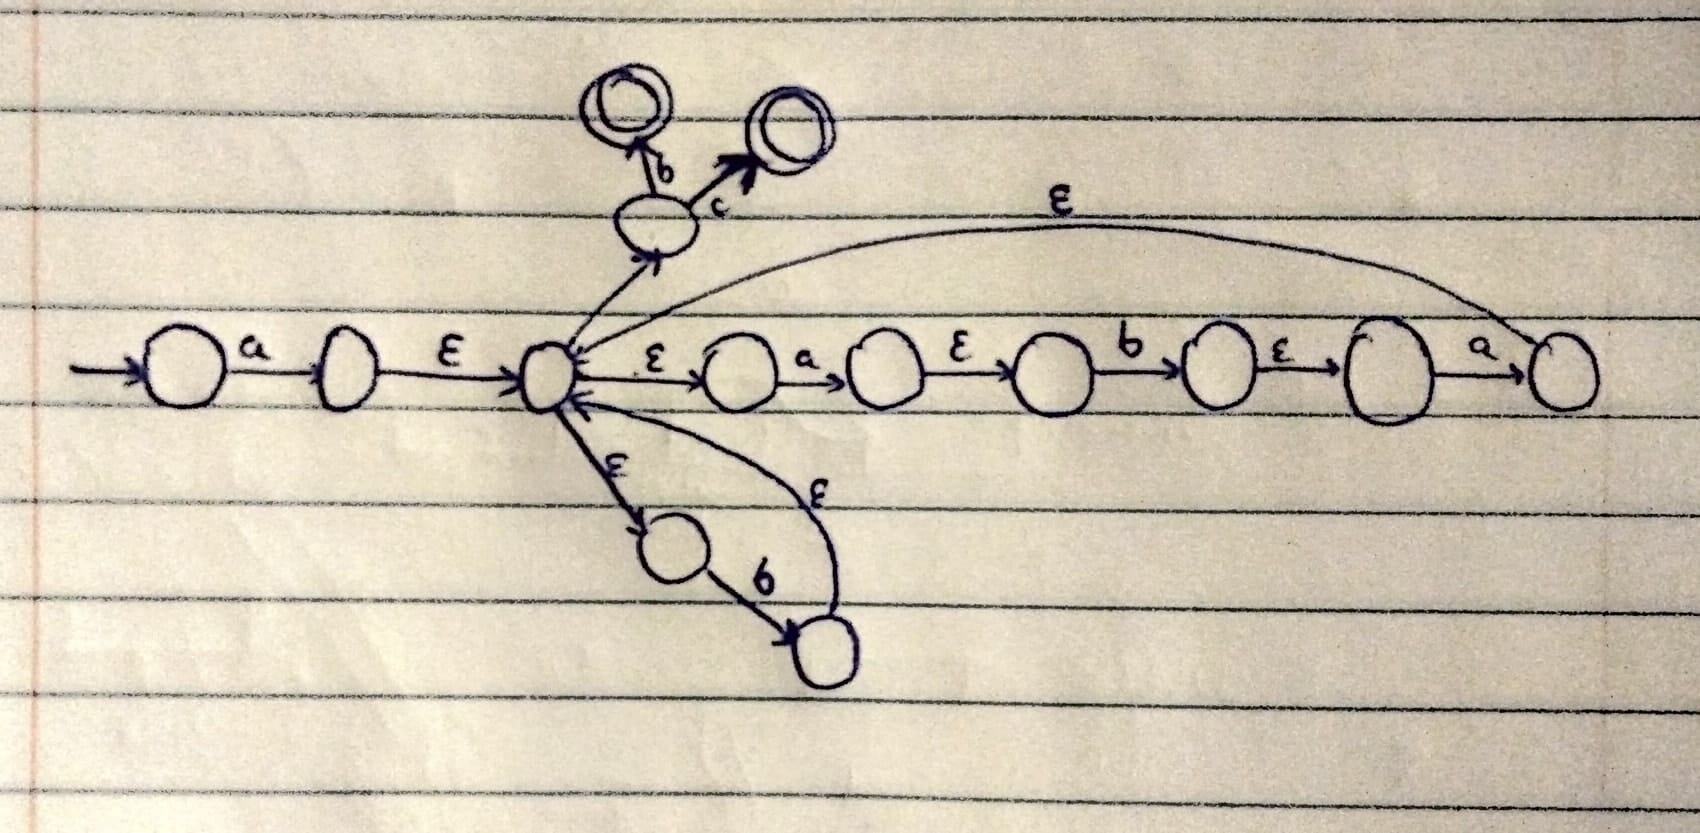
\includegraphics[scale = 0.20]{4}


\end{document}